\documentclass[10pt]{article}

\usepackage[utf8]{inputenc}
\usepackage[T2A]{fontenc}
\usepackage[russian,english]{babel}

\usepackage{amssymb,textcomp,tabularx,graphicx}

\title{Задание 1}
\author{Коновалов Андрей, 074}
\date{}

\let\eps\varepsilon

\begin{document}

\maketitle

\noindent
\newcolumntype{C}{>{\centering\arraybackslash}X}%
\begin{tabularx}{\textwidth}{|C|C|C|C|C|C|C|C|}
\hline
1 & 2 & 3 & 4 & 5.1 & 5.2 & 6 & $\sigma$ \\
\hline
&&&&&&& \\
\hline
\end{tabularx}

\bigskip

{\bf Задача 1}

{\bf 1.}
Докажем что $L \subseteq T$ индукцией по количеству конкатенаций $n$. Пустое слово $\eps \in L$ и $\eps \in T$, поэтому докажем включение, учитывая слова ненулевой длины.

{\em База.}
Все слова, полученные с помощью одной конкатенации, т.е. слова вида $bax, baax, bbax, bbaax$, где $x = \eps$, принадлежат языку $T$, поскольку начинаются с $a$, заканчиваются на $b$, и не имеют подслов $aaa$ и $bbb$. База доказана.

{\em Переход.}
Пусть слова, полученные с помощью $n$ конкатенаций принадлежат языку $T$. Докажем, что слова полученные с помощью $n + 1$ конкатенации принадлежат языку $T$.

Каждое слово $w \in L$, полученное после $n + 1$ конкатенации состоит из префикса $p \in \{ba, baa, bba, bbaa\}$ и суффикса $s \in T$. Заметим, что $p$ начинается с $b$, а $s$, по предположению индукции, заканчивается на $a$. Получаем, что $w$ начинается c $b$ и заканчивается на $a$. Поскольку $p$ заканчивается на $a$, а $s$ начинается с $b$, а также $p$ и $s$ не содержат подслов $aaa$ и $bbb$, то слово $w = ps$ не содержит подслов $aaa$ и $bbb$. Получаем, что слово $w \in T$. Переход доказан.

{\bf 2.}
Докажем, что $T \subseteq L$ индукцией по длине слова $n$.

{\em База.}
Посмотрим на словa, принадлежащие языку $T$ длины $0 \leq n \leq 4$. Они представляют собой множество $W = \{ \eps, ba, baa, bba, baba, bbaa\}$. Заметим, что $W \subseteq L$. База доказана.

{\em Переход.} 
Пусть слова длины меньше $n$ принадлежат языку $L$. Докажем, что слова длины $n$ принадлежат языку $L$. Поскольку база была доказана для $0 \leq n \leq 4$, то при доказательсте перехода будем считать, что $n \geq 5$.

Каждое слово $w \in T$ должно начинаться с $b$ и не может иметь подслово $bbb$. Следовательно префикс  длины $3$ слова $w$ может быть лишь: $baa$, $bab$ или $bba$. Разберем эти три случая.

Если $baa$ является префиксом, то следующей буквой после этого префикса может быть лишь $b$, поскольку иначе существовало бы подслово $aaa$. Получаем, что $baab$ является префиксом. В этом случае $w = baa  \cdot x$, где $x \in L$ по предположению индукции. Следовательно $w \in L$.

Если $bab$ является префиксом, то $w = ba \cdot x$, где $x \in L$ по предположению индукции. Следовательно $ w \in L$.

Если $bba$ является префиксом, то возможны $2$ случая: префиксом является $bbab$ или $bbaa$. В первом случае $w = bba \cdot x$, где $x \in L$ по предположения индукции. Следовательно $w \in L$. Во втором случае префиксом является $bbaab$, поскольку $bbaaa$ содержит подслово $aaa$ и не может быть префиксом. Получаем, что $w = bbaa \cdot x$, где $x \in L$ по предположения индукции. Следовательно $w \in L$. Переход доказан.

{\bf 3}
Используя пункты 1 и 2 и соответственно факты $L \subseteq T$ и $T \subseteq L$ получаем, что $L = T$.

\medskip

{\bf Задача 2}

{\bf 1.}
Заметим, что $a \in \{ a^{5n+1} | n \geq 0\}$. Следовательно $\{ a^{5n+1} | n \geq 0\}^* = \{ a^{n} | n \geq 1\} = \{ a \}^*$. Следовательно $\{ a^{3n} | \, n>0\} \cap \{ a^{5n+1} | n \geq 0\}^* = \{ a^{3n} | \, n>0\} \cap \{ a \}^* = \{ a^{3n} | \, n>0\}$.

{\bf 2.}
В пересечение множеств входят только те элементы, которое входят в оба множества. Но в пустое множество не входит ни одного элемента, следовательно $\emptyset \cap \{\eps\} = \emptyset$.

{\bf 3.}
Заметим, что в $h^{-1}(L)$ входят лишь слова $x$ в алфавите $\{ a, b \}$, такие что $3 |x|_a + 2 |x|_b = 7n$ для некоторого $n \geq 0$, поскольку $h(a) = aaa$ и $h(b) = aa$, и никакие другие. Значит, $h^{-1}(L) = \{ x \in \{ a, b \}^* | 3 |x|_a + 2 |x|_b = 7n | n \geq 0 \}$.

\medskip

{\bf Задача 3}

{\bf 1.}
Докажем, что равенство ложно. Рассмотрим $L = \{ \eps, a \}$ в алфавите $\{ a \}$. Рассмотрим $h$: $h(\eps) = \eps$, $h(a) = \eps$. Заметим, что $h^{-1}(L) = \{ a^n | n \geq 0 \}$. А значит $h(h^{-1}(L)) = \{ \eps \} \neq L$.

{\bf 2.}
Докажем, что равенство ложно. Рассмотрим $L = \{ a^n | n \geq 0 \}$ в алфавите $\{ a, b \}$. Рассмотрим $h$: $h(\eps) = \eps$, $h(a) = a$, $h(b) = a$. Заметим, что $h(L) = L$. Заметим, что $h^{-1}(L) = \{ x \in \{ a, b \}^* | |x|_a + |x|_b = n \} \neq L$. А значит $h^{-1}(h(L)) = h^{-1}(L) \neq L$.

\medskip

{\bf Задача 4}

{\bf 1.}
${\cal A}$ является детерминированным, поскольку для $\forall$ вершины $\nexists$ двух исходящих из нее ребер, помеченных одинаковой буквой.

{\bf 2.}
Последовательность конфигураций: $(q_0, 011001) \vdash (q_0, 11001) \vdash (q_1, 1001) \vdash (q_0, 001) \vdash (q_0, 01) \vdash (q_0, 1) \vdash (q_1, \eps)$. Поскольку $q_1$ - финальное состояние, то $w\in L({\cal A})$.

{\bf 3.}
Последовательность конфигураций: $(q_0, 001100) \vdash (q_0, 01100) \vdash (q_0, 1100) \vdash (q_1, 100) \vdash (q_0, 00) \vdash (q_0, 0) \vdash (q_0, \eps)$.

{\bf 4.}
Слова $\{ 1, 01 \} \in L({\cal A})$. Последовательности конфигураций для них: $(q_0, 1) \vdash (q_1, \eps)$ и $(q_0, 01) \vdash (q_0, 1) \vdash (q_1, \eps)$ соответственно.

Слова $\{ \eps, 0 \} \notin L({\cal A})$. Последовательности конфигураций для них: $(q_0, \eps)$ и $(q_0, 0) \vdash (q_0, \eps)$ соответственно.

\medskip

{\bf Задача 5.1}

{\bf 2.}
Докажем, что автомат ${\cal A}$, заданный в задаче 4 принимает язык $L_4$ по индукции по длине слова $n$. А именно докажем, что после обработки слова, которое дает остаток $i$ при делении на $3$, ${\cal A}$ будет находится в состоянии $q_i$ (в соответствии с обозначениями в условии). Соответственно слова, которые представляют собой числа, дающие остаток $1$ при делении на $3$, будут переводить ${\cal A}$ в состояние $q_1$, которое является финальным. Поскольку каждому слову сопоставляется число, далее будем говорить про слова, как про числа. Также, далее, при упоминании остатка, имеется ввиду остаток при делении на $3$.

{\em База.}
Заметим, что слово $\eps$ не принимается ${\cal A}$. Посмотрим на слова $\{ 0, 1 \}$ длины $n = 1$. После обработки слова $0$, дающее остаток 0, ${\cal A}$ перейдет в состояние $q_0$, а после обработки слова $1$, дающее остаток $1$ - в состояние $q_1$. База доказана.

{\em Переход.}
Пусть после обработки любого слова длины меньше $n$, дающего остаток $i$, ${\cal A}$ находится в состоянии $q_i$. Докажем, что для всех слов длины $n$ это тоже выполняется.

Посмотрим на произвольное слово $x$ длины $n$. Представим его ввиде: $x = y \cdot a$, где $y$ - слово длины $n - 1$, $a \in \{ 0, 1 \}$. Заметим, что $x = 2_{10} \cdot y + a$. Обозначим остаток числа $t$: $r(t)$. Заметим, что $r(x) = r(2_{10} \cdot r(y) + a)$.

Дадим ${\cal A}$ обработать слово $y$.

Пусть сейчас ${\cal A}$ находится в состоянии $q_0$, и, соответственно, $r(y) = 0$. Если $a = 0$, то $r(x) = 0$, а ${\cal A}$ перейдет в состояние $q_0$. Если $a = 1$, то $r(x) = 1$, а ${\cal A}$ перейдет в состояние $q_1$. В обоих случаях доказываемое свойство выполняется.

Пусть сейчас ${\cal A}$ находится в состоянии $q_1$, и, соответственно, $r(y) = 1$. Если $a = 0$, то $r(x) = 2$, а ${\cal A}$ перейдет в состояние $q_2$. Если $a = 1$, то $r(x) = 0$, а ${\cal A}$ перейдет в состояние $q_0$. В обоих случаях доказываемое свойство выполняется.

Пусть сейчас ${\cal A}$ находится в состоянии $q_2$, и, соответственно, $r(y) = 2$. Если $a = 0$, то $r(x) = 1$, а ${\cal A}$ перейдет в состояние $q_1$. Если $a = 1$, то $r(x) = 2$, а ${\cal A}$ перейдет в состояние $q_2$. В обоих случаях доказываемое свойство выполняется.

Все случаи разобраны, в каждом из них доказываемое свойство для слова $x$ выполняется. Переход доказан. 

\medskip

{\bf Задача 6.}

{\bf 2.}
Докажем, что автомат ${\cal A}$, изображенный на диаграмме ниже, является искомым. $q_0$ - начальное состояние. $q_{1a}$ и $q_{2a}$ - финальные состояния. Заметим, что если ${\cal A}$ пришел в нефинальное состояние $q_2$, то он из него уже не выйдет и текущее слово не может быть принято.

\noindent 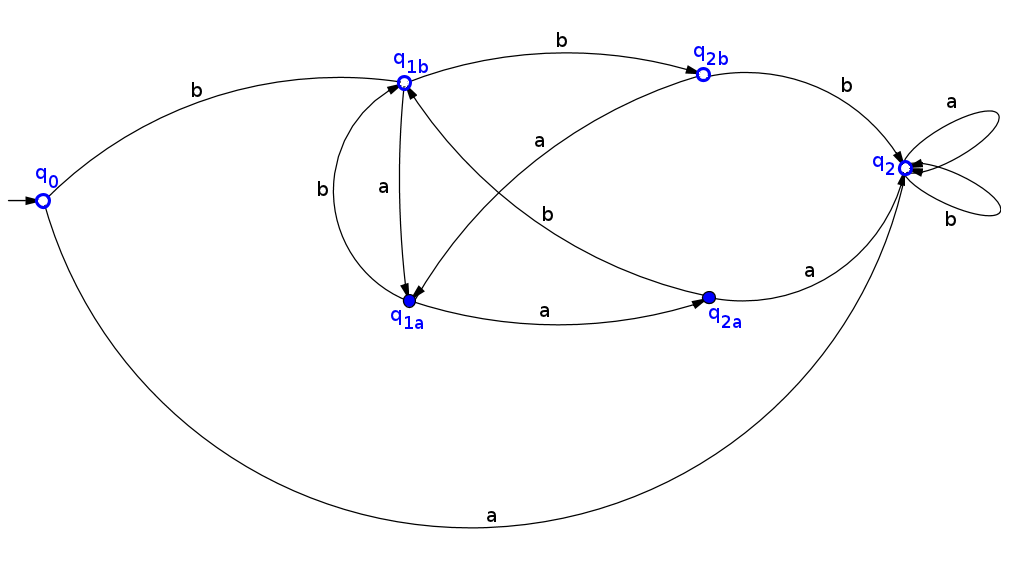
\includegraphics[width=\textwidth]{alpha.png}

Сначала докажем, что ${\cal A}$ принимает слова из языка $T$. Первой буквой любого слова из языка $T$ является $b$. Это означает, что после ее обработки ${\cal A}$ перейдет в состояние $q_{1b}$. Далее ${\cal A}$ в состояние $q_0$ уже не вернется, поскольку в него не входит ни одно ребро.

Докажем, что, после обработки слова из языка $T$, ${\cal A}$ не может оказаться в состоянии $q_2$. Заметим, что в $q_2$ можно попасть только из $q_{2b}$ по букве $b$ или из $q_{2a}$ по букве $a$. В состояние $q_{2b}$ можно попасть только из состояния $q_{1b}$, перейдя по букве $b$, в которое, в свою очередь, можно попасть только по букве $b$. Это означает, что, что бы перейти в состояние $q_2$ по букве $b$, что бы $3$ последние обработанные буквы были буквами $b$. Аналогично, что бы перейти в состояне $q_2$ по букве $a$, надо, что бы $3$ последние обработанные буквы были буквами $a$. Но любое слово из $T$ не содержит подслов $aaa$ и $bbb$. 

Это означает, что после окончания обработки слова из языка $T$, ${\cal A}$ окажется в одном из состояний: $q_{1b}$, $q_{2b}$, $q_{1a}$ или $q_{2a}$. Поскольку последней буквой слова из $T$ всегда является $a$, то ${\cal A}$ закончит исполнение в одном из состояний: $q_{1a}$ или $q_{2a}$, поскольку только в них можно перейти по букве $a$. А эти состояния являются финальными, а значит ${\cal A}$ принимает слова из языка $T$.

Теперь докажем, что ${\cal A}$ не принимает никакие другие слова. Поскольку из $q_0$ существует ребро в $q_2$ подписанное буквой $a$, то быть принятым может лишь слово, начинающееся с буквы $b$. Также, поскольку в финальные состояния входят лишь ребра, подписанные буквой $a$, то слово, оканчивающееся на $b$ принято быть не может. Заметим, что если в слове встречается подслово $aaa$ или подслово $bbb$, то после его обработки ${\cal A}$ перейдет в состояние $q_2$, в каком бы состоянии он до этого не находился.

Получаем, что ${\cal A}$ принимает язык $T$.

{\bf 3.}
Заметим, что после обработки первой буквы слова, ${\cal A}$ перейдет в состояние $q_2$, и далее из него не выйдет. Последовательность конфигураций: $(q_0, abbabbbabbabbbabbbababbabba) \vdash (q_2, bbabbbabbabbbabbbababbabba) \vdash^* (q_2, \eps)$.

\end{document}
